\subsection{Introduction}
在搜索或推荐领域, 准确率通常是我们想到的第一个目标, 但真的是这样吗? 说到底, 各个平台的最终目的是为提供令用户更满意的服务, 为平台留住用户, 创造更多的利益. 为达成这些目的, 准确率够吗?

就视频推荐而言, 以单个目标作为优化对象的问题:
\begin{myitemize}
	\item 目标偏差: 点赞, 分享表达的满意度比播放更高;
	
	\item 物品偏差: 不同视频的播放时长体现的满意度不一致;
	
	\item 用户偏差: 有的用户偏向于点赞, 而有的偏向于收藏.
\end{myitemize}

选择哪个目标来进行优化才能满足我们的要求呢? 一个比较直接的方式就是同时优化所有的目标: 1) 单目标难以直接衡量用户满意度, 多目标优化可以最大限度地利用丰富的隐式反馈数据建模用户满意度; 2) 推荐系统排序模块要求低时延, 多目标优化训练一个模型可以预测多个目标, 线上融合多目标的预测结果进行排序.


多目标任务的常用模型: 
\begin{myitemize}
	\item MOE(Mixture-of-Experts), \textcolor{red}{1991};
	\item Shared-Bottom, \textcolor{red}{1997};
	\item ESMM, SIGIR'2018;
	\item MMoE, KDD'2018;
	\item SNR(Subnetwork Routing), AAAI'2019;
	\item PLE, RecSys'2020;
	\item AITM, KDD'21;
\end{myitemize}

多任务学习通常通过 Hard 或 Soft 参数共享来完成: 
\begin{myitemize}
	\item 共享 Hard 参数是神经网络 MTL 最常用的方法, 可以追溯 1993 年 Caruana 所发表的论文. 在实际应用中, 通常通过在所有任务之间共享隐藏层, 同时保留几个特定任务的输出层来实现. 共享Hard 参数大大降低了过拟合的风险. 1997 年 Jonathan Baxter 在他的论文中证明过拟合共享参数的风险为 O(N)——其中 N 是任务数——小于过拟合特定任务参数, 即输出层. 这很直观: \textbf{同时学习的任务越多, 模型找到一个含有所有任务的表征就越困难, 而过拟合原始任务的可能性就越小};
	
	\item 另一方面, 在共享 Soft 参数时, 每个任务都有自己的参数和模型. 模型参数之间的距离是正则化的, 以便鼓励参数相似化. 1998 年 Caruana 对早期的 MTL 的研究进行了总结, 并演示了三个领域中的多任务学习. 他们解释了多任务学习的工作原理, 提出了一个基于案例的方法 (如 kNN 和核回归) 的多任务学习算法和结果, 并为决策树中的多任务学习绘制了一个算法. 目前大部分MTL学习所基于的机制仍然来源于此篇文章.
\end{myitemize}
 

MTL 通常受到数据分布以及任务之间相关性的影响 (\textbf{如何衡量任务之间的相关性、关系}) . 

\subsection{多目标任务的技巧}
\subsubsection{样本加权}
在优化主目标的同时, 将其他目标转化为样本权重, 借此来达到优化其他目标的效果. 例如主目标为 CTR, 同时还有一个目标是停留时长. 则可以给停留时长长的样本赋予更高的权重. 

\textbf{特点}: 这种方式模型简单, 上线容易, 仅在训练时通过梯度乘以权重实现对其他目标的加权即可. 但本质上不是多目标建模, 而是将多个目标转化为一个目标, 目标的加权权重需要根据线上 A/B 测试才能确定. 而且, 可能不适用于多个从目标的情况, 因为将多个从目标转化为样本权重很难找到一个合适的平衡. 

\subsubsection{模型融合}
多目标模型融合, 通过将一个模型同时训练多个目标 (label 的构造) . 该方法的优点是各个任务之间能够共享信息, 同意迭代方便, 节省资源. 缺点: 目标越多模型越复杂, 各个任务之间相互影响, 迭代速度慢. 


\subsection{ESMM}
ESSM, Entire Space Multi-task Model, 诞生于阿里于 2018 年在 SIGIR 上发表的论文 "Entire Space Multi-Task Model: An Efficient Approach for Estimating Post-Click Conversion Rate". 该论文针对 CVR 估计中的样本选择偏差 (Sample Selection Bias, SSB) 和 数据稀疏 (Data Sparsity, DS) 问题, 提出了一个多任务学习的模型, 模型结构如 Fig.\ref{fig:esmm} 所示.

\begin{figure}[h]
	\centering
	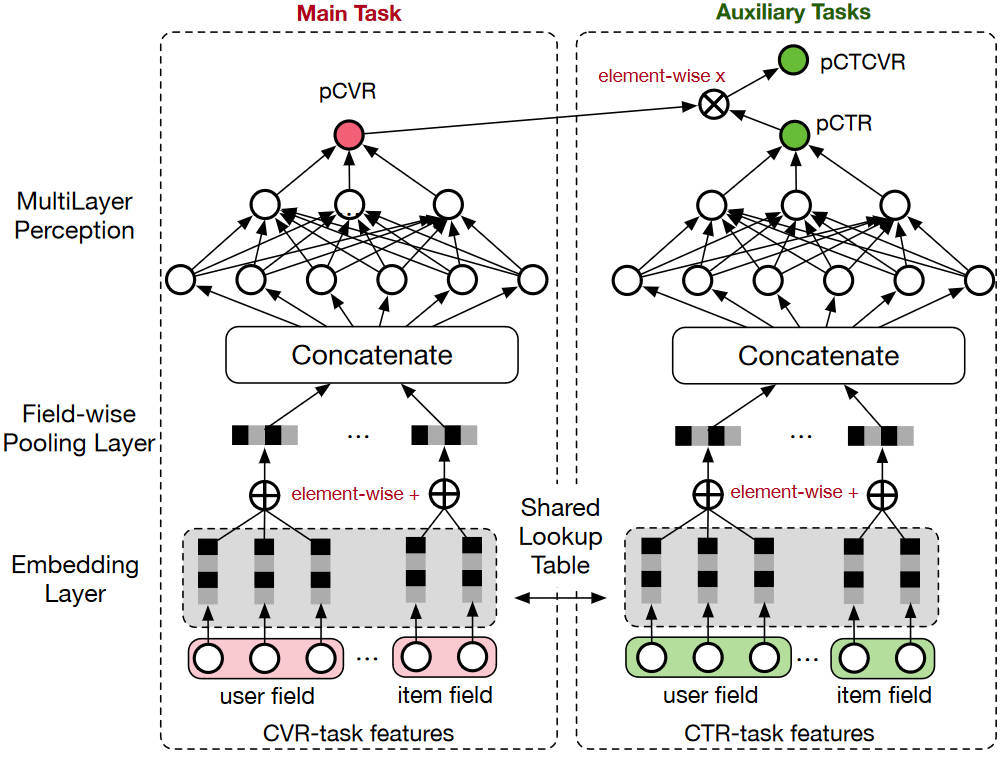
\includegraphics[width=\textwidth]{pics/esmm.jpg}
	\caption{The structure of ESMM}
	\label{fig:esmm}
\end{figure}

\subsubsection{Motivation}
转化率预估(CVR)目前主要存在两个难点: 
\begin{itemize}
	\item SSB. 从 CVR 模型使用的角度来看, 其训练过程是\textcolor{red}{有偏}的. CVR 预估模型是\textbf{在点击的样本上进行训练的}, 但是被用于\textcolor{red}{在整个样本空间上进行推断}. 这样做实际上存在一个问题, 训练和预测的数据分布的不一致会损害模型的泛化能力;
	
	\item DS. 实际上CTR预估的数据就已经非常稀疏了, 点击后再转化的数据则更少了;
\end{itemize}

ESMM(Entire Space Multi-Task Model) 并没有直接在整个样本空间上去预估CVR, 而是采用两个辅助的任务: CTR 和 CTCVR 来间接的预测 CVR, 而不是直接通过在点击数据上训练 CVR 模型, 因为这些数据是有偏的, 如果直接用其余样本作为负样本, \textbf{并不知道这些没被转化是因为没被点击还是因为其他原因}.

\subsubsection{HOW}
\begin{figure}[h]
	\centering
	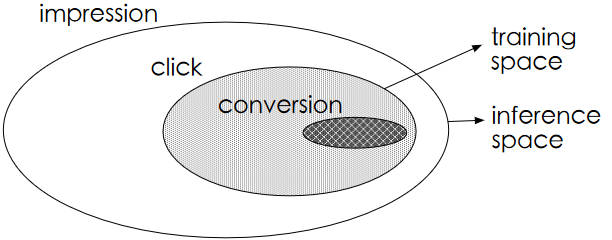
\includegraphics[width=.5\textwidth]{pics/ssb.jpg}
	\caption{Illustration of sample selection bias problem in conventional CVR modeling. Training space is composed of samples with clicked impressions. It is only part of the inference space which is composed of all impressions.}
	\label{fig:ssb}
\end{figure}

结合 Fig.\ref{fig:esmm} 来看, \textit{Main Task} 是 pCVR, 两个辅助任务是 pCTR, pCTCVR, 被估计的样本是 $x$. 先看看各个任务的\textbf{训练样本}是什么:
\begin{itemize}
	\item pCTR: 曝光样本空间, 即 Fig.\ref{fig:ssb} 中的 impression, 曝光中点击的 ($y=1$) 作为正样本, 未点击的作为负样本;
	
	\item pCVR: 点击空间, 即 Fig.\ref{fig:ssb} 中的click, 转化的 ($z=1$) 作为正样本, 未转化的作为负样本;
	
	\item pCTCVR: 曝光空间, 点击且转化的 ($y=1\&z=1$) 作为正样本;
\end{itemize}
要注意: \textbf{\textcolor{red}{pCVR 是在整个曝光空间上推断时}} --- SSB 问题的来源. 那能不能在整个曝光空间上来训练 pCVR 呢? 回顾一下 ESMM 的名字 "\textbf{Entire Space} Multi-Task Model", 重点在于这个 Entire Space, 这个空间指的就是 Fig.\ref{fig:ssb} 中的 impression. 其实这也回答了刚刚的问题, 可以在整个曝光空间上训练 pCVR. 那就来看看 ESMM 怎么做的.

ESMM 中并不直接去估计 pCVR, 而是去估计 pCTR 和 pCTCVR. 这两个辅助任务的训练空间都是曝光空间. 这两个辅助任务与主任务之间的关系:
$$
\underbrace{p(y=1, z=1 \mid x)}_{p C T C V R}=\underbrace{p(y=1 \mid x)}_{p C T R} \times \underbrace{p(z=1 \mid y=1, x)}_{p C V R}
$$

如 Fig.\ref{fig:esmm} 所示, ESMM 由两个子网络组成, 左边的估计 pCVR, 右边的估计 pCTR, 二者相乘得到 pCTCVR, 实际训练时只针对 pCTR 和 pCTCVR 计算损失:
$$
\begin{aligned}
	L\left(\theta_{c v r}, \theta_{c t r}\right) &=\sum_{i=1}^{N} l\left(y_{i}, f\left(x_{i} ; \theta_{c t r}\right)\right) \\
	&+\sum_{i=1}^{N} l\left(y_{i} \& z_{i}, f\left(x_{i} ; \theta_{c t r}\right) \times f\left(x_{i} ; \theta_{c v r}\right)\right)
\end{aligned}
$$
ESMM 的目的是训练一个能够在全样本空间上进行 CVR 估计的模型, 但是并没有直接去训练这个模型的参数, 而是通过 pCTR, pCTCVR 与 pCVR 之间的约束关系 $pCTCVR = pCTR * pCVR$ 来学习 pCVR 模型的参数. 其实, 也可以分别单独估计 pCTR 和 pCTCVR 再来求 pCVR, 但是这样会有两个问题: 1) CTR, CTCVR 都是很小的数, 做除法会有数值上的不稳定, 而且 2)单独估计时二者之间不存在约束关系, 做除法时可能会得到大于 1 的 CVR.

\subsubsection{总结}
\begin{itemize}
	\item ESMM 通过多任务学习来解决 CVR 样本空间在训练和推理时不一致的问题, 利用了 CVR, CTR 这两个目标之间的依赖关系;
	
	\item ESMM 这种形式可以推广到目标\textbf{具有依赖关系}的场景中, \textcolor{red}{对于关系比较模糊的场景该怎么办呢?}
	
	\item 真实场景中, 可以直接使用 CVR 的模型来进行打分作为排序的依据;
\end{itemize}

\subsection{Shared-Bottom}
简称为 SB, 即多个任务之间有一个共享的底座. SB 是由 Rich Caruana 与 1997 年在其博士论文中提出来的. SB 有一个被多个任务共享的模块 (shared-bottom network), 该模块的输出作为各个任务的输入, 每个任务有一个单独的网络来学习. SB 对任务相关性高的多任务学习效果较好, 也能加速训练进程的收敛, 但是当任务的目标不相关甚至相反时, 可能会影响各个任务的学习效果.

\subsection{MMoE}
MMoE, Multi-gate Mixture-of-Experts, 诞生于 Google 于 2018 年八月在 KDD 上发表的论文 "Modeling Task Relationships in Multi-task Learning with Multi-gate Mixture-of-Experts". 基于 NN 的多任务学习模型一般对任务之间的关系比较敏感, 即在相关性强的任务上效果好, 相关性弱的效果差. 该论文提出了 MMoE 来克服任务间关系敏感的问题.

\subsubsection{Motivation}
在很多场景中, 通常是要同时考虑多个目标的, 一开始大家都是未每个任务建一个模型, 但是随着数据量和业务规模的扩大和复杂化, 一个任务一个模型的成本越来越高, 效果也不太稳定. 那么能不能同时对所有任务一起建模, 一起学习和优化呢? 当然是可以的, 这方面的尝试也早就开始了 --- multi-task learning. 但有时多任务学习的效果并不如单个模型独立学习, 这里面是有很多原因造成的, 例如任务之间的相关性, 差异性. 其中一个主要的原因就是\textcolor{red}{\textbf{任务间的关系 / 差异}}, 这也是大家研究的较多的一个方向. 为什么任务间差异大效果就不好呢? 由于任务间差异大, 可能各个任务的最优解是相距很远的, 甚至是互斥的. 以往的工作为了弥补任务间的差异, 会引入更多的参数, 这样做会增加学习的计算量, 而且在真实的场景中有些参数是不可获得的.

\subsubsection{HOW}

\begin{figure}[h]
	\centering
	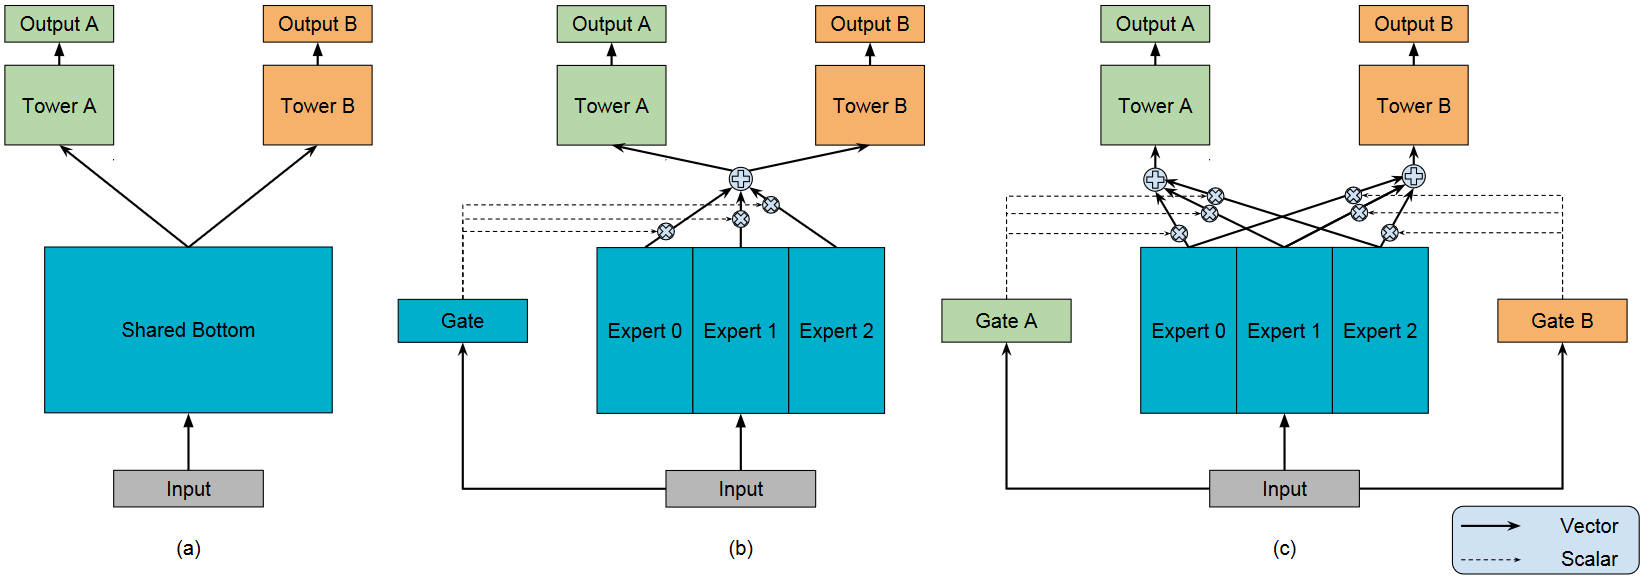
\includegraphics[width=.85\textwidth]{pics/mmoe.jpg}
	\caption{(a) Shared-Bottom model. (b) One-gate MoE model. (c) Multi-gate MoE model.}
	\label{fig:mmoe}
\end{figure}

MMoE 的模型结构如 Fig. \ref{fig:mmoe} (c) 所示. 可以看到, 这三个模型是有明显的递进关系的, 从 SB 的单个 shared-bottom 到 MoE 的多个 shared-bottom, 从 MoE 的单门控到 MMoE 的多门控. 从 SB, MoE 可以看出, 人物之间的差异出要体现在 Task-specific 的那部分参数. 虽然 MoE 中引入了一个 gating network, 但是对不不同的 Task-specific 模块来说, 输入依然是一样的 (有点残差的意思). 再看 MMoE, 除了 Task-specific 的输出模块, 还有 Task-specific 的 gating network. 形式化地定义一下 MMoE 中每个任务的输出:
$$
\begin{aligned}
	y_k &= h^k (f^k (x)) \\ 
	f^k (x) &= \sum_{i=1}^n g^k (x)_i f_i(x)  \\
	g^k (x) &= softmax(W_{gk} x)
\end{aligned}
$$
其中 $k$ 表示第 $k$ 个任务, $n$ 是 Experts 的数量. $g^k \in \mathbb{R}^n$ 表示针对 $k$ 的 gating network, $f_i$ 是 MoE 中第 $i$ 个 Expert 的输出, \textbf{是一个向量}, $h^k$ 则是 $k$ 的输出模块, $f^k$ 是 $k$ 的输出模块的输入. 很显然, MMoE 在 MoE 的基础上, 为每个任务引入了一个 gating network.

\textcolor{red}{为什么为每个任务加一个 gating network 有效呢?} 首先看看门控的作用. 每一个门控相当于对专家网络的选择 / 开关, 对于不同的 $x$ 就像打开了不同的开关. 而不同门控之间的关系则隐含了不同任务之间的关系.

\subsubsection{总结}
\begin{itemize}
	\item 通过 Multi-gate 隐式地建模了不同任务之间的关系, 且对任务之间的关系鲁棒;
	
	\item 不同的 Expert 学习不同的信息, 不同的 gating network 学习任务特定的信息以将 Expert 学到的信息进行组合;
\end{itemize}